\documentclass[12pt]{article}

% margins and page style
\usepackage[margin=2.5cm]{geometry}
\usepackage{fancyhdr}
\pagestyle{fancy} 

% spaces between paragraphs
\usepackage[parfill]{parskip}

% fonts
\usepackage[T1]{fontenc}
\usepackage[scaled=0.92]{helvet}
\renewcommand*\familydefault{\sfdefault}

% font size of section headings
\usepackage{sectsty}
\sectionfont{\fontsize{14}{15}\selectfont}

% tables 
\usepackage{booktabs}
\renewcommand{\arraystretch}{1.5}

% figures
\usepackage{graphicx}
\usepackage[font=small,labelfont=bf]{caption} 

% colors
\usepackage[dvipsnames,svgnames,hyperref,table]{xcolor}

% hyperlinks
\usepackage{hyperref}
\hypersetup{
  pdfauthor={Erin C. McKiernan},
  colorlinks=true,
  urlcolor=Bittersweet,
  linkcolor=blue,
  citecolor=Purple,
}

% bib options
\let\oldbibliography\thebibliography
\renewcommand{\thebibliography}[1]{\oldbibliography{#1}
\setlength{\itemsep}{0pt}} 
\usepackage[numbers,sort&compress]{natbib} 
\bibliographystyle{unsrtnat}

% title and authors
\usepackage{authblk}
\title{\vspace{-1.8cm}\Large{\textbf{Electrocardiography basics: recording the electrical activity of the heart before and after exercise}}}
\author[1]{Erin C. McKiernan}
\affil[1]{\small{Departamento de F\'isica, Facultad de Ciencias, Universidad Nacional Aut\'onoma de M\'exico}}

\date{}

%%%%%%%%%%%%%%%%%%%%%%%%%%%%%%%%%%%%%%%%%%%%%%%%%%%%%%%%%%%%
 
\begin{document}
\maketitle

\section*{OVERVIEW}
In this laboratory practical, students will learn how the heart works
as a pump, and how this function is related to the electrical activity
of different cells in the heart. Students will learn about the basics
of electrocardiography, and record their
electrocardiograms at rest and after exercise to see how the heart
rhythm changes with activity. Overall, this practical will help
students to better understand carviovascular physiology and the
importance of electrical signals in the heart.

\section*{SPECIFICATIONS}
\begin{tabular}{p{6cm} p{10cm}}
\textbf{Level of study:} & Undergraduate \\
\textbf{Degree programs:} & Biology, Physics, Biomedical Physics, others \\
\textbf{Semester:} & 4th (i.e. 2nd year undergrads) \\ 
\textbf{For use in courses:} & Systems Physiology, others \\
\textbf{Recommended prior courses:} & Molecular \& Cellular Biology \\
\textbf{Duration of practical:} & 1-2 hours \\
\textbf{Setting:} & Classroom or laboratory \\
\textbf{Safety considerations:} & Students should not eat for at least 30 minutes prior, have water and chairs available for rest after physical activity \\
\textbf{Other indications:} & Wear loose clothing to permit electrode placement
\end{tabular}

\section*{OBJECTIVES}
\textbf{Before doing this lab you should be able to:}
\begin{itemize}
\item describe the basic anatomy of the heart
\item identify the different cell types in the heart
\item understand the basics of action potential generation in excitable cells
\item understand the basics of heart muscle contraction
\end{itemize}
 
\vspace{0.3cm}

\textbf{In this lab you will:}
\begin{itemize}
\item learn how to record electrocardiagrams (ECGs)
\item identify and measure the different waves and intervals in the ECG 
\item observe and record changes in the ECG before and after physical activity
\end{itemize}

\vspace{0.3cm}
 
\textbf{After doing this lab you should be able to:}
\begin{itemize}
\item explain the relationship between heart cell electrical activity and heart function
\item understand the basics of ECG recording
\item design further experiments to investigate the activity of the heart under different conditions or in combination with other recordings
\end{itemize}

\section*{EQUIPMENT}

\begin{itemize}
\item Heart \& Brain SpikerShield with integrated Arduino (Backyard Brains)
\item 3 surface electrodes (Backyard Brains or other provider)
\item cable with alligator clips to connect electrodes to SpikerShield (Backyard Brains)
\item USB cable to connect SpikerShield to computer (Backyard Brains)
\item Computer with free Backyard Brains SpikeRecorder software installed (note that a smartphone or tablet will not work, since cable connects to USB port)
\end{itemize}

\section*{BACKGROUND}

\subsection*{The heart as a pump}

The principal function of the heart is to pump blood. In fact, the heart can be thought of as a system of two pumps working in sync: one pump that sends blood to the lungs to be oxygenated, and another that pumps blood to the rest of the body to provide oxygen and nutrients to tissues and organs \cite{khanHeart,mohrman2006cardiovascular}. Why is the pumping action of the heart necessary? Why not simply allow gases and nutrients to travel by diffusion to tissues and organs? We know from Fick's Law that the rate of diffusion is inversely proportional to distance \cite{khanHeart,sperelakis2012cell}. Therefore, diffusion works well over short distances, but is far too slow to be physiologically effective over large distances. We need the heart and its pumping action to get blood quickly to destinations that are large distances away. Once there, the short distances within tissues and organs facilitate gas and nutrient exchange.

Each time the heart pumps blood it does external mechanical work \cite{mohrman2006cardiovascular,khanWork}. In fluid systems, the work performed is given by

\begin{equation}
    \textrm{Work} = \textrm{Pressure of the fluid x Volume of the fluid}
\end{equation}

In the case of the heart, we are interested in the work done with each heart beat, called the stroke work, which is calculated by multiplying the pressure of the blood by the volume of blood moved (stroke volume). We can visualize the pressure and volume changes as the heart pumps with a pressure-volume loop \cite{khanPV} (Fig. \ref{fig:pvLoop}).

\begin{figure}[h!]
\centering
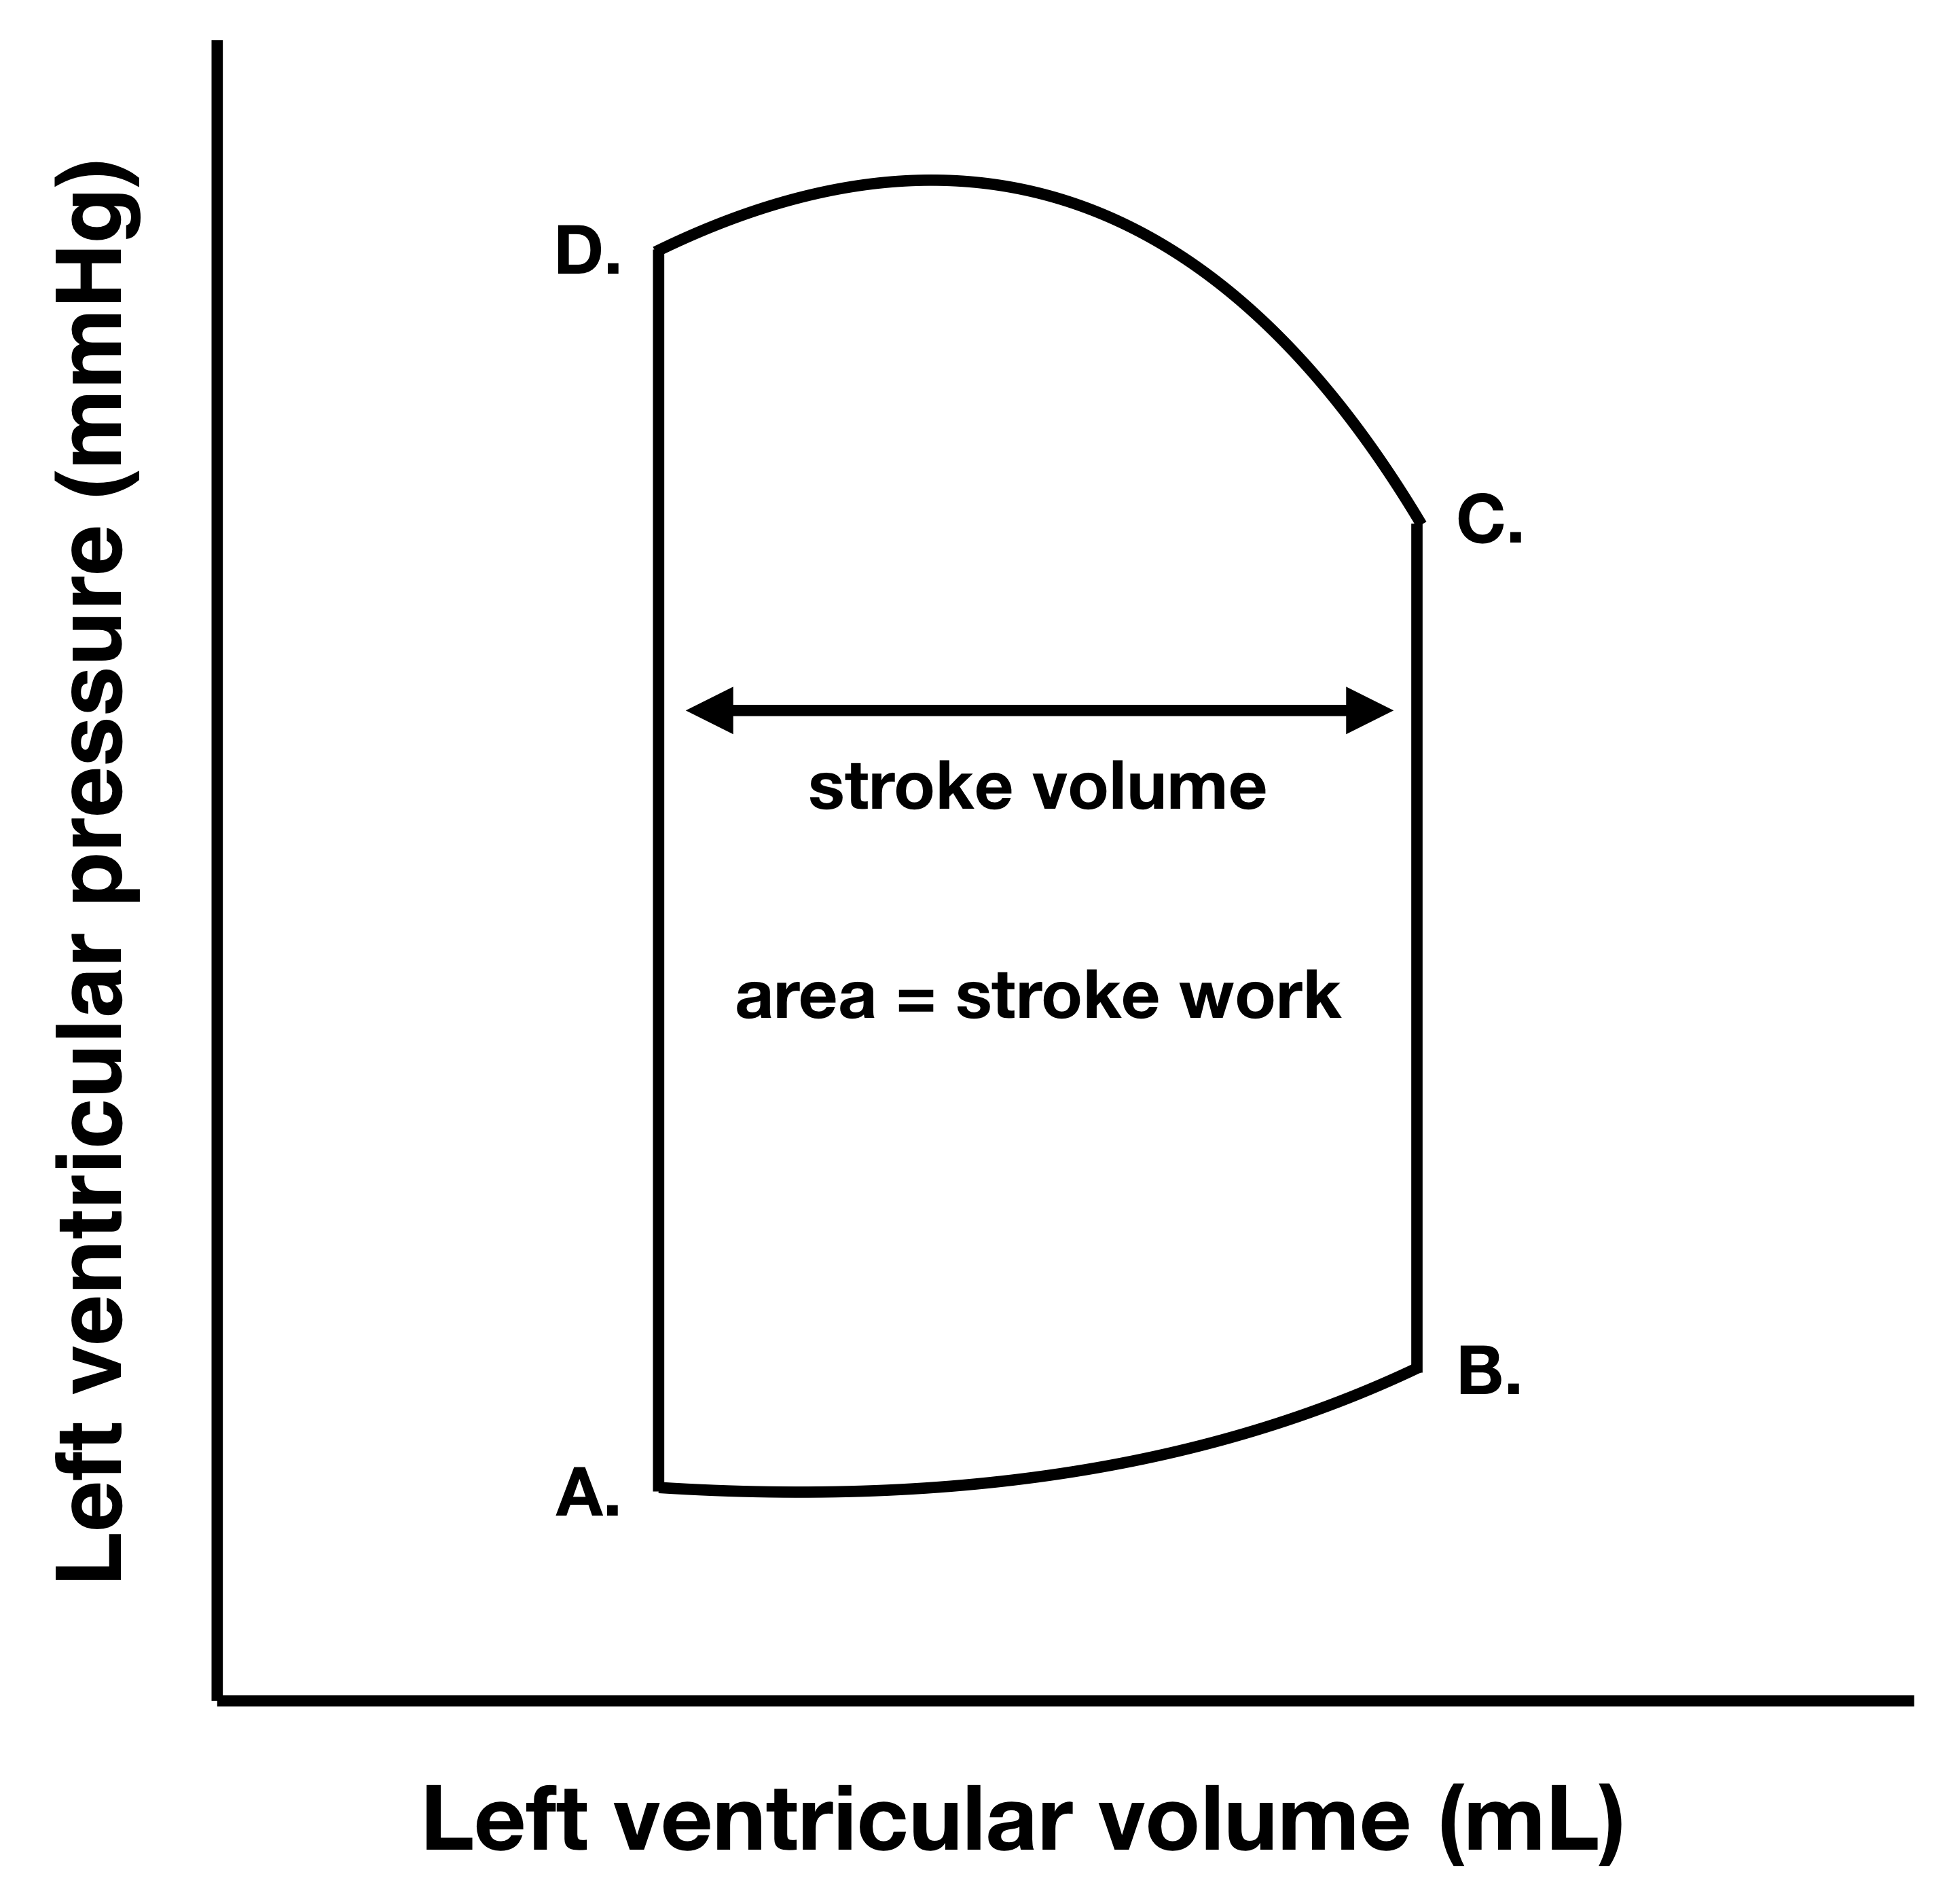
\includegraphics[width=0.7\textwidth]{figures/pvLoop.png}
\caption{Pressure-volume loop for the left ventricle. Image: Erin C. McKiernan, CC BY.}
\label{fig:pvLoop}
\end{figure}

For simplicity, we can start by modeling the heart as a ``single-chamber pump'' with inflow and outflow valves \cite{khanWork}. At point A. in Fig. \ref{fig:pvLoop}, the inflow valve opens and the chamber fills with blood, increasing the volume. At B., the inflow valve closes and a force is exerted on the blood in the chamber (we will see later that this force is due to heart muscle contraction). Because the blood cannot escape the chamber while the valves are closed, pressure rises. Eventually, the pressure is sufficient to open the outflow valve (C.) and blood exits the heart. At D., the outflow valve closes again, muscle relaxes, force is no longer exerted on the blood, and the pressure drops. The difference between points B. and A. gives the stroke volume, while the area inside the loop equals the stroke work. Pressure-volume loops can be used to assess the function of the heart under different conditions, or to diagnose diseases where the pumping of the heart may be compromised. For more information and practice exercises, see \cite{khanPV}.

\subsection*{Anatomy of the heart}

To understand more about the function of the heart, it is important to go beyond the single-pump chamber model and look in detail at its anatomy (Fig. \ref{fig:heart}). The heart has four chambers -- two atria in the upper region of the heart and two ventricles in the lower region \cite{mohrman2006cardiovascular,khanHeart,openStaxHeart}. Blood that has circulated throughout the body and is now low in oxygen arrives to the right side of the heart via the superior and inferior vena cavae, filling the right atrium. Blood that has just been oxygenated in the lungs returns to the heart via the pulmonary vein, filling the left atrium. 

Blood flow from the atria to the ventricles is controlled by valves. The tricuspid valve controls flow from the right atrium to the right ventricle, while the mitral valve controls flow from the left atrium to the left ventricle. Flow from the ventricles is also controlled by valves. The pulmonary valve controls flow from the right ventricle through the pulmonary artery, while the aortic valve controls flow from the left ventricle through the aorta. Blood within the right ventricle exits the heart via the pulmonary artery, which carries blood to the lungs to be oxygenated. Blood within the left ventricle exits the heart via the aorta and circulates to the rest of the body \cite{mohrman2006cardiovascular,khanHeart,openStaxHeart}. 

\begin{figure}[h!]
\centering
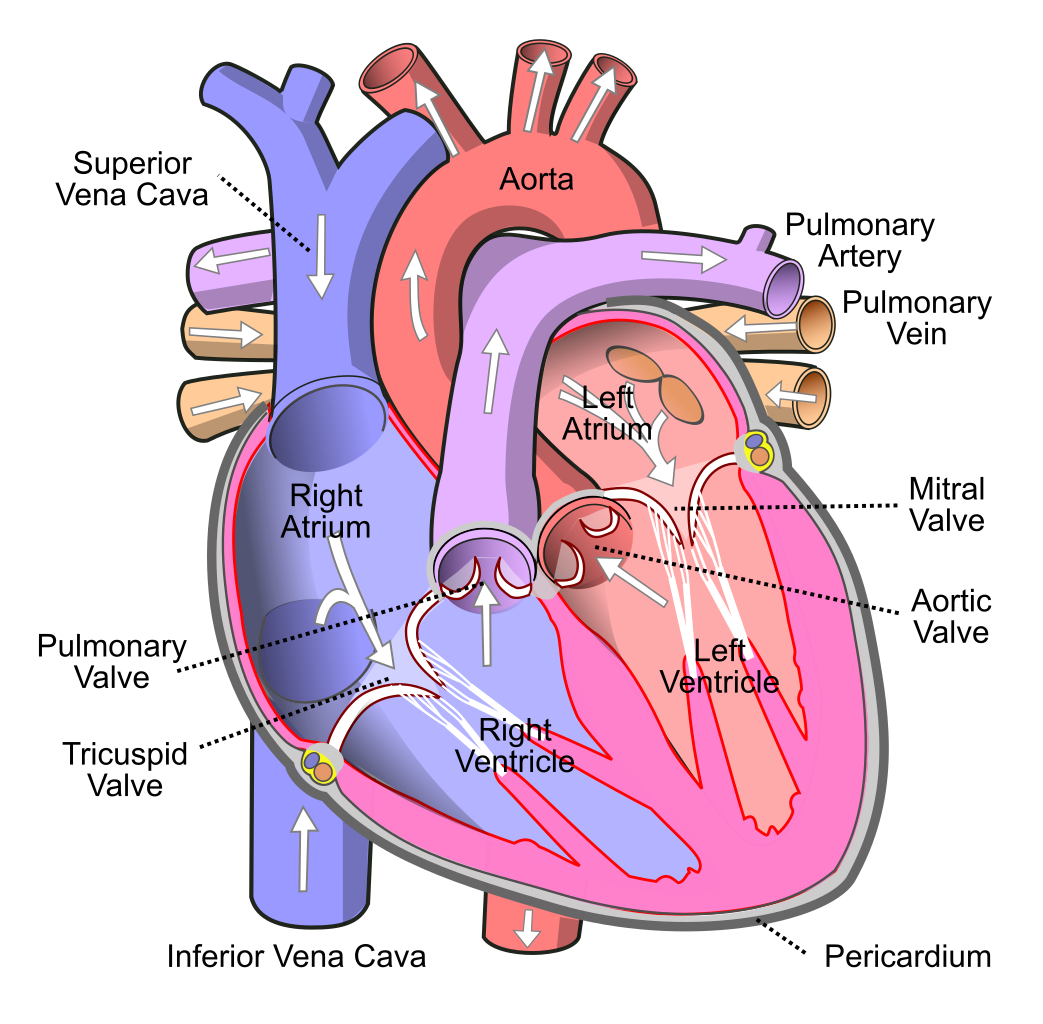
\includegraphics[width=0.65\textwidth]{figures/heart.png}
\caption{Anatomy of the heart. Image: Wapcaplet via Wikimedia Commons, CC BY-SA.}
\label{fig:heart}
\end{figure}

\subsection*{Cardiac cycle}

The sequence of events that occur with each heart beat to pump blood between the chambers and eventually out of the heart is called the cardiac cycle \cite{openStaxCycle,guyton2016book}. The cardiac cycle can be divided into two principal phases, systole and diastole. In general, diastole refers to a period when the musculature of a given chamber relaxes and the chamber fills with blood, while systole occurs when the musculature contracts and blood is ejected from the chamber. Both the atria and ventricles undergo systole and diastole, but these occur at different times. 

The cardiac cycle begins with both the atria and ventricles in diastole, i.e. relaxed and filling with blood (Fig. \ref{fig:cycle}). At this time, since the tricuspid and mitral valves are open, blood can flow freely from the atria to the ventricles and fill the latter up to 80\% \cite{guyton2016book,openStaxCycle}. Next, while the ventricles are still in diastole, the atria enter into systole, contracting and ejecting the remaining blood into the ventricles to complete filling. Once the ventricles are full, the tricuspid and mitral valves close and the ventricles start to contract, marking the beginning of ventricular systole. Since all the heart valves are closed, and because we know that liquids are largely incompressible \cite{mccall2010physics}, ventricular contraction during this period occurs isovolumetrically (at constant volume) and intraventricular pressure rises. 

\begin{figure}[h!]
\centering
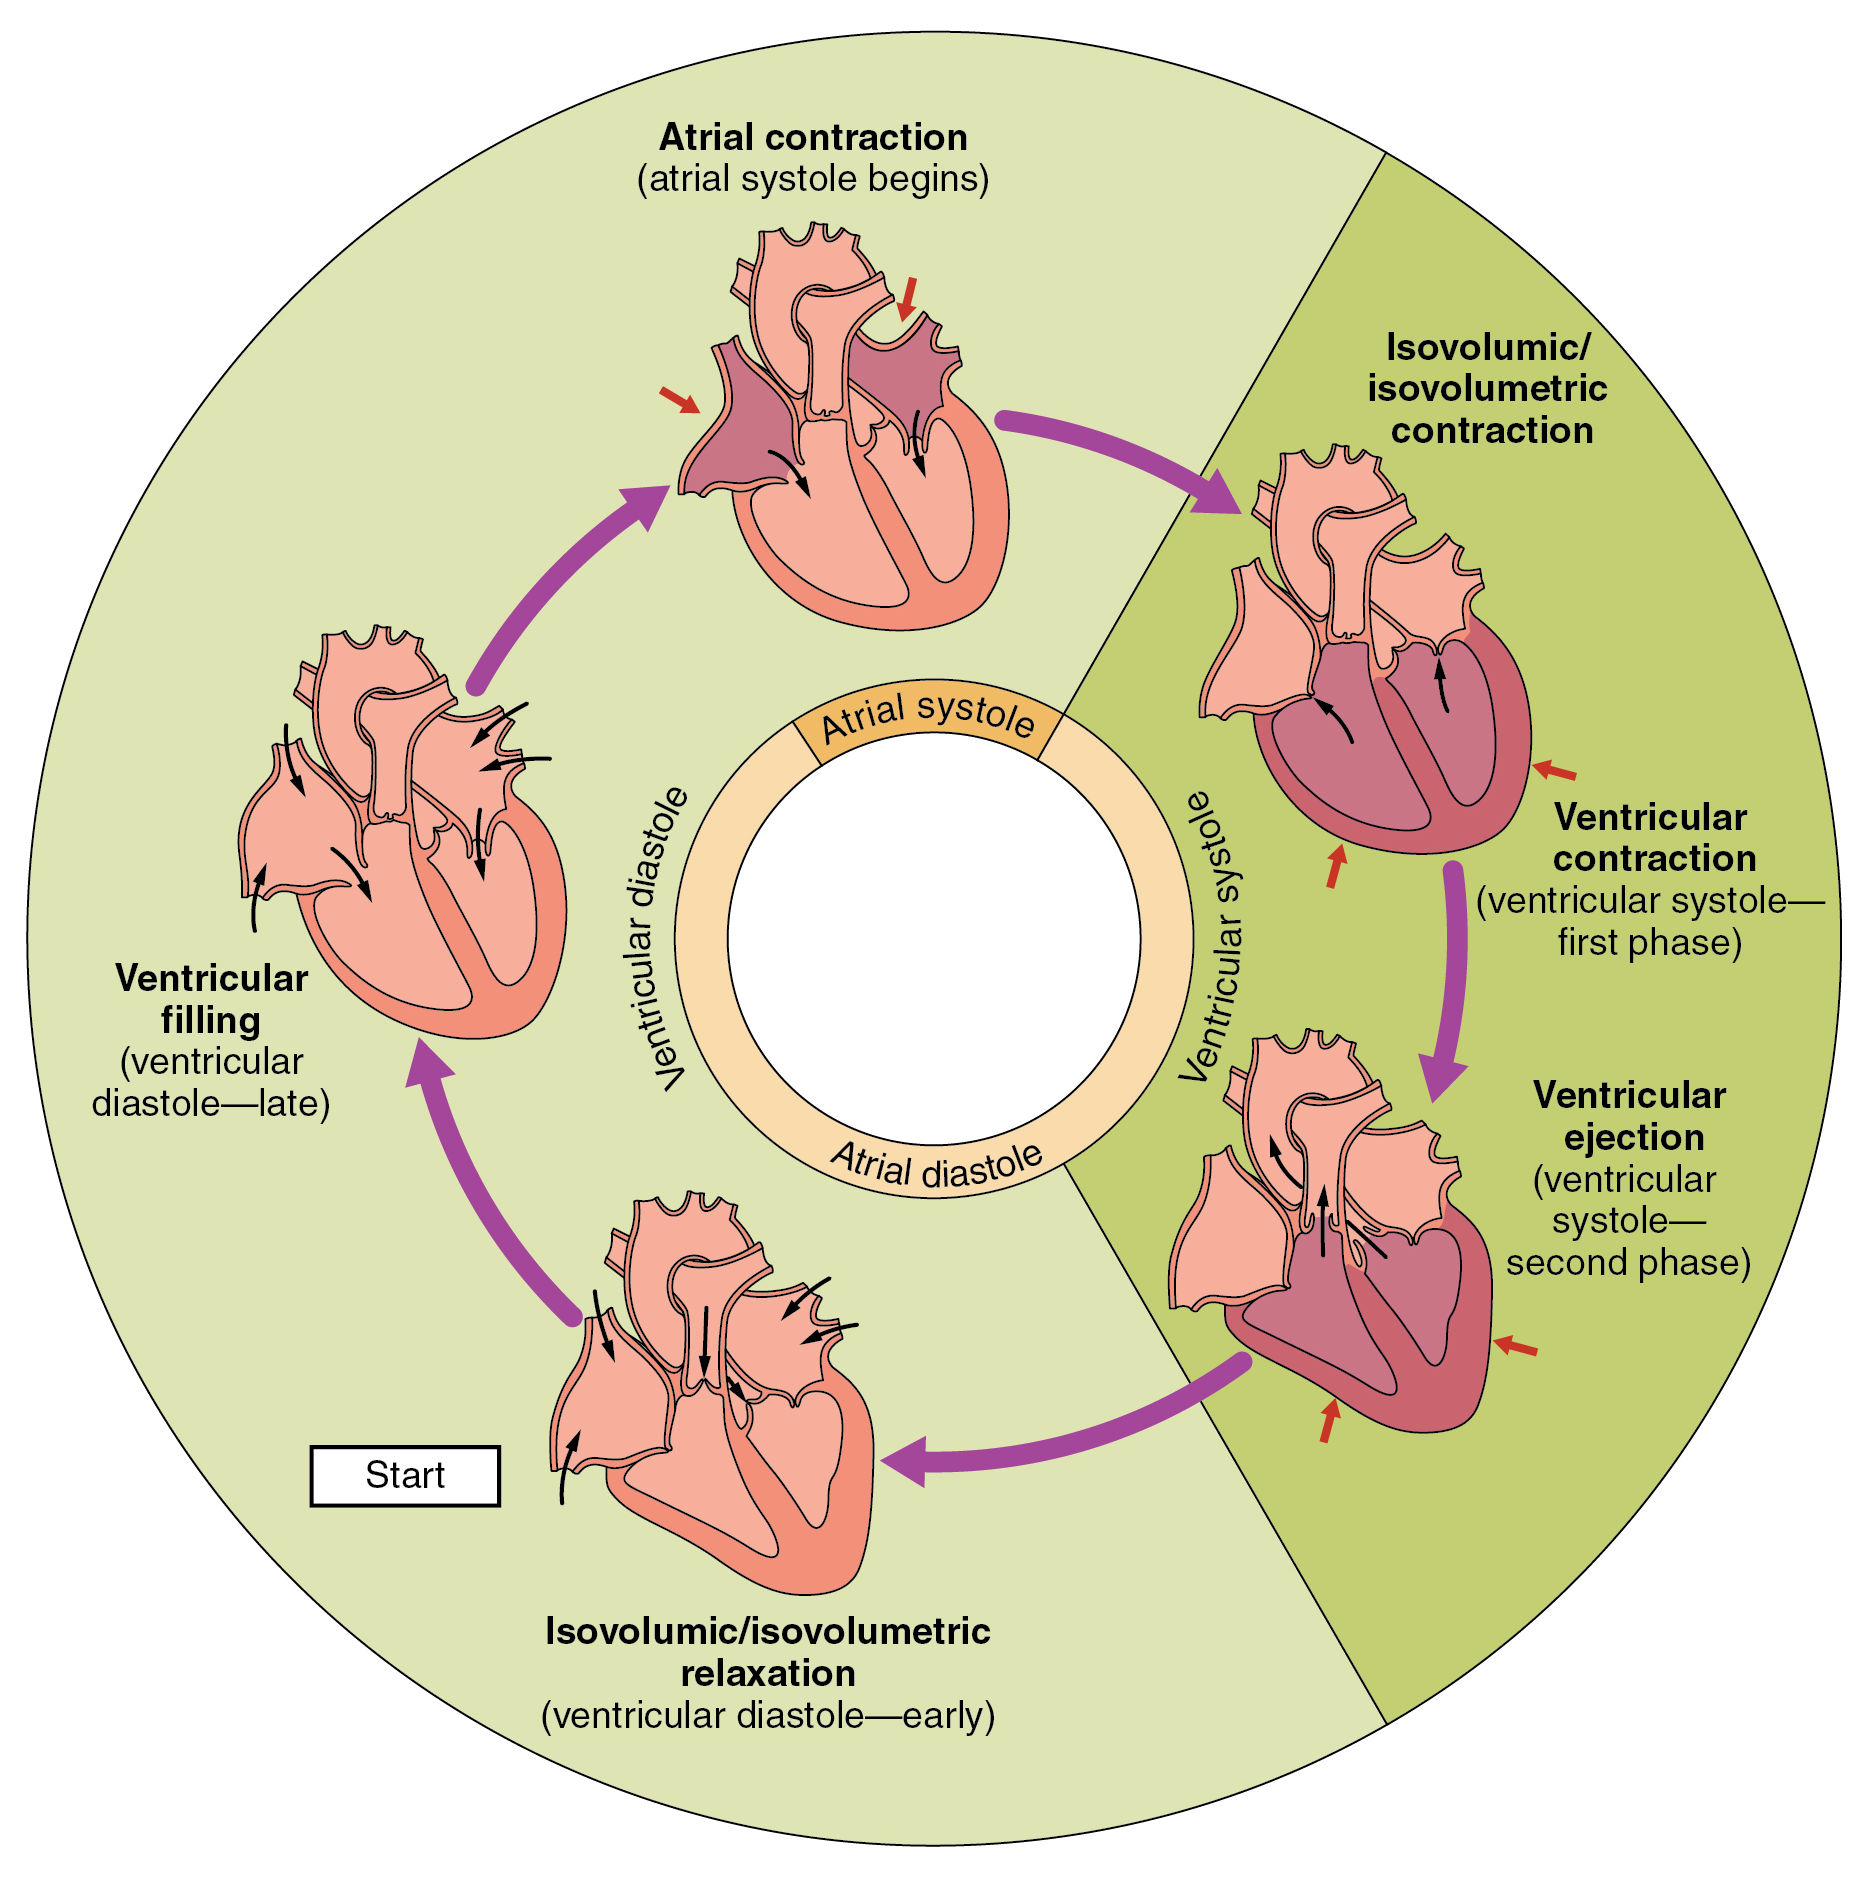
\includegraphics[width=0.7\textwidth]{figures/cardiacCycle.png}
\caption{Events of the cardiac cycle. Image: OpenStax College \citep{openStaxCycle}, CC BY.}
\label{fig:cycle}
\end{figure}

As ventricular contraction continues, the pressures in the right and left ventricles rise above the pressures in the pulmonary artery and aorta, respectively. This allows the pulmonary and aortic valves to open, and blood is ejected from the heart. As blood exits the ventricles and the musculature relaxes, the ventricles return to diastole and the pressure drops, causing the pulmonary and aortic valves to close. With all valves closed, the ventricles relax isovolumetrically at first. However, when the ventricular pressure drops below the atrial pressure, the tricuspid and mitral valves open and blood flows from the upper to lower chambers, and the cycle begins again \cite{guyton2016book,openStaxCycle}. 

\subsection*{Electrical activity in the heart}

\subsubsection*{Nodal and conducting cells}
  
The electrical signals which drive rhythmic muscle contractions in the heart originate in the sinoatrial (SA) node \cite{openStaxElectrical,mohrman2006cardiovascular}, which is located in the upper right atrium (Fig. \ref{fig:conduction}). 

\begin{figure}[h!]
\centering
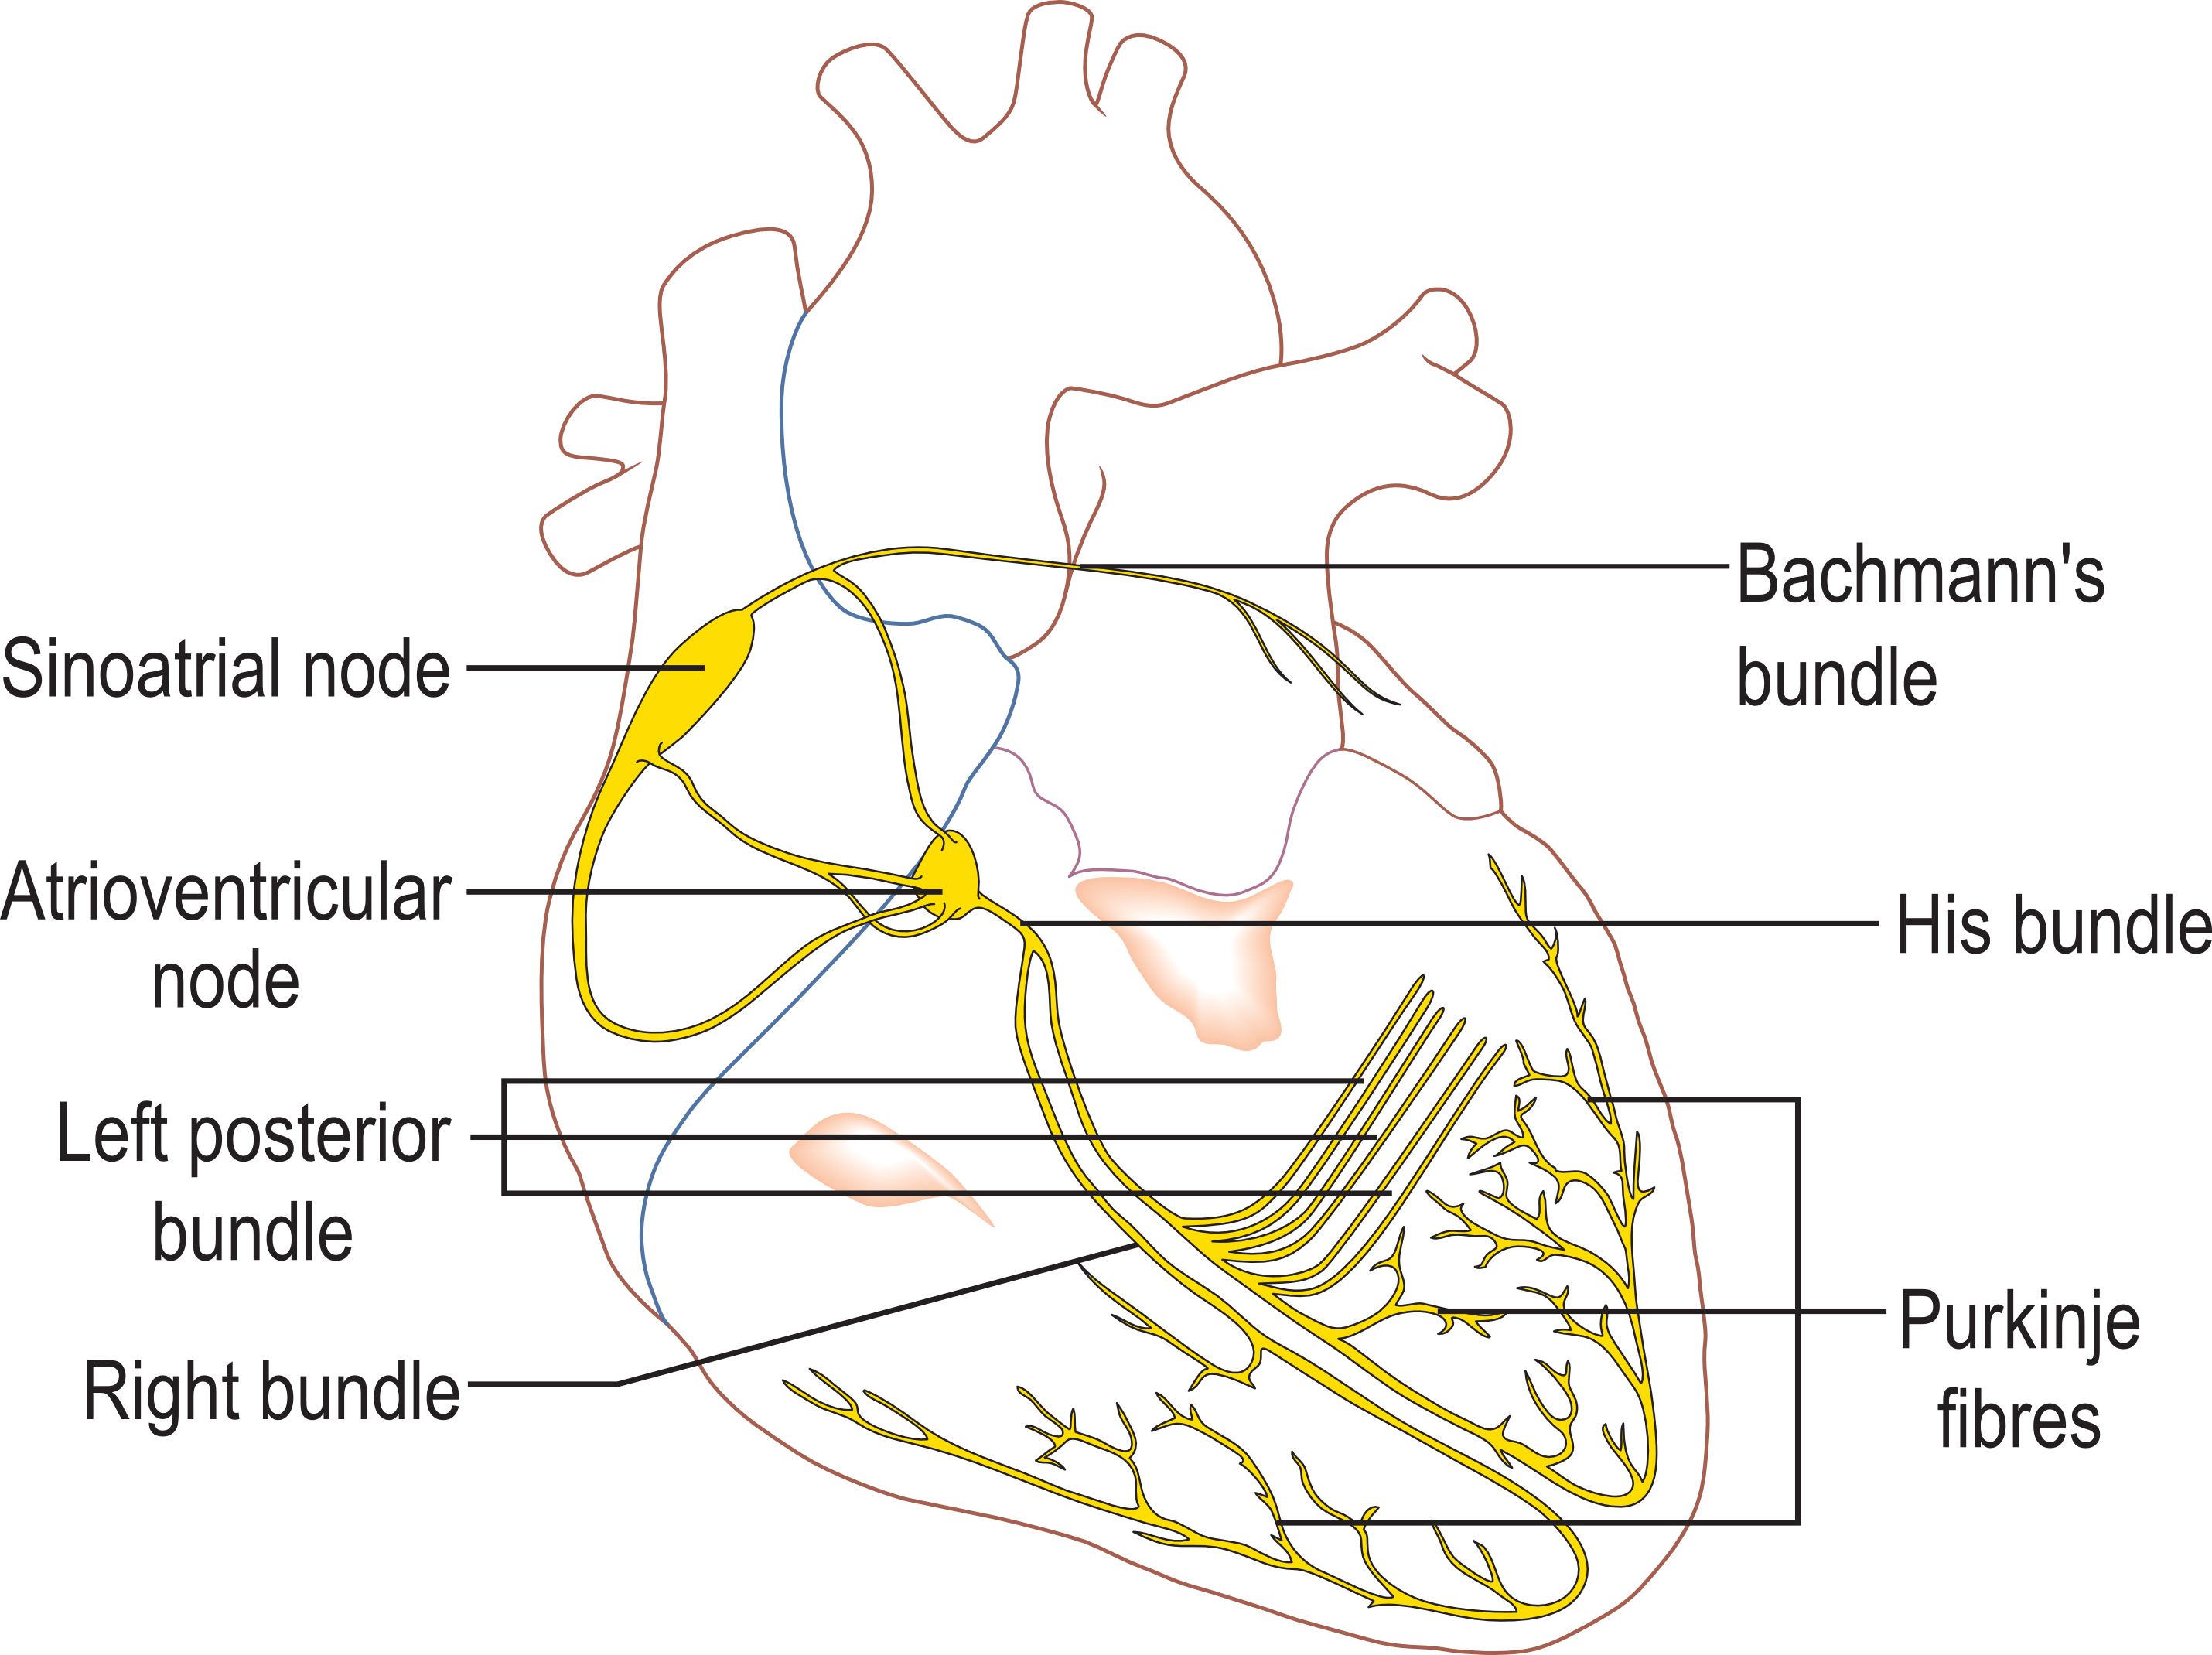
\includegraphics[width=0.85\textwidth]{figures/conduction.png}
\caption{Electrical conduction system in the heart. Image: Madhero88 via Wikimedia Commons, CC BY.}
\label{fig:conduction}
\end{figure}

In the SA node, a group of special myocardial cells self-generate regular electrical impulses called action potentials (APs), thereby acting as pacemakers. Unlike many excitable cells, SA node cells do not have a resting membrane potential \cite{openStaxElectrical,mohrman2006cardiovascular}. Instead, their membrane potential continuously varies due to the interplay of different calcium, sodium, and potassium currents  (Fig. \ref{fig:nodeAP}). The upstroke of the AP is caused when calcium channels in the cell membrane open, allowing calcium to enter the cell down its electrochemical gradient, depolarizing the cell. Shortly after, potassium channels open, allowing these ions to exit the cell along their gradient, repolarizing the cell. Once the membrane potential reaches hyperpolarized values ($\sim$ -60 mV), channels which carry primarily sodium ions open and allow these ions to enter the cell, causing it to slowly depolarize. This small, primarily sodium-based current has been called the `pacemaker current' or the `funny current' \cite{difrancesco2012funny}. Once this slow depolarization brings the membrane potential within a certain voltage range, calcium channels open again and generate another AP. In this way, the ion channel dynamics sustain regular, rhythmic AP firing. While nodal cells can generate pacemaking activity without nervous system input, the frequency of their firing can be regulated by the autonomic nervous system \cite{openStaxElectrical,mohrman2006cardiovascular}.

\begin{figure}[h!]
\centering
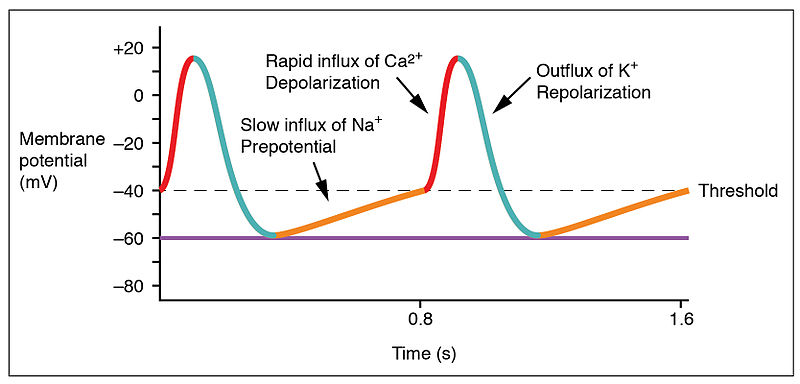
\includegraphics[width=0.85\textwidth]{figures/pacemaker.jpg}
\caption{Pacemaker AP firing in nodal cells. Image: OpenStax \citep{openStaxElectrical}, CC BY.}
\label{fig:nodeAP}
\end{figure}
 
Electrical impulses generated in SA nodal cells propagate to a similar set of cells in the atrioventricular (AV) node \cite{openStaxElectrical,mohrman2006cardiovascular}, located in the lower part of the right atrium (Fig. \ref{fig:conduction}). AV nodal cells produce APs similar to those seen in SA nodal cells (Fig. \ref{fig:nodeAP}) and are capable of taking over pacemaking activity, if necessary \cite{feher2012quantitative,guyton2016book}. Under normal conditions, however, AV cells receive input from SA cells that drive the rhythm. The conduction time between the two nodes serves as a delay to allow myocytes in the atria to depolarize before signals are sent to the ventricles, and helps maintain the different phases of the cardiac cycle.

APs produced in AV nodal cells travel first down the bundle of His, then to each ventricle via the right and left bundle branches, and finally to the Purkinje fibers, which spread throughout the ventricular walls \cite{openStaxElectrical,feher2012quantitative}. Collectively, the above components make up the electrical conduction system of the heart, responsible for carrying signals quickly to contractile myocytes to produce coordinated contraction and efficient pumping action.

\subsubsection*{Contractile myocytes}

Around 99\% of cells in the heart are contractile myocytes \cite{openStaxElectrical}. These are the muscle cells that contract to develop tension and accomplish the pumping action of the heart.

The action potentials generated in contractile myocytes are different than those generated in nodal cells \cite{mohrman2006cardiovascular,openStaxElectrical}. Unlike in nodal cells, where the upstroke is due primarily to calcium influx, the upstroke in contractile cells results from sodium influx (Fig. \ref{fig:ventAP}). Shortly after opening, sodium channels close and inactivate, leading cells to briefly repolarize slightly (note the notch in the AP in Fig. \ref{fig:ventAP}). However, calcium channels soon open, allowing these ions to enter and keep the cell depolarized for a prolonged period ($\sim$100-200 ms), creating a plateau potential. Finally, the calcium channels close, and that together with potassium efflux repolarizes the cell. Contractile cells, unlike nodal cells, do have a resting membrane potential, which is close to the potassium equilibrium potential \cite{mohrman2006cardiovascular,openStaxElectrical}. These cells are not typically auto-rhythmic like nodal cells, but fire regularly due to the rhythmic input they receive from the nodal cells via the electrical conduction system.

\begin{figure}[h!]
\centering
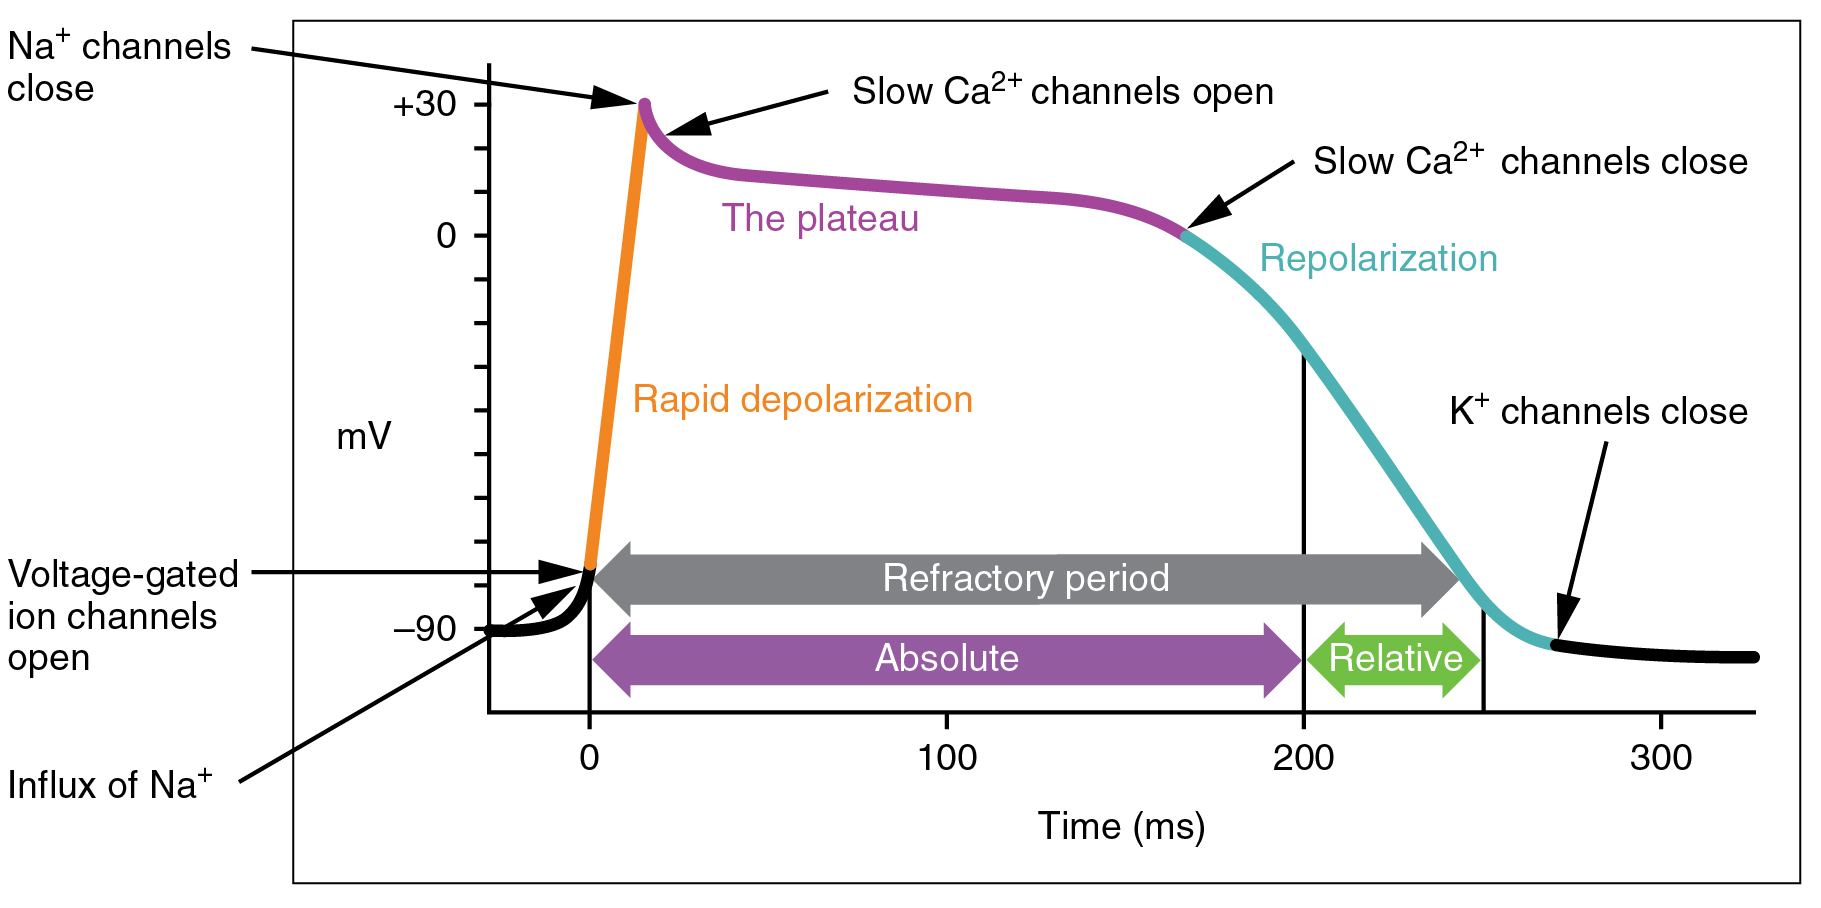
\includegraphics[width=0.85\textwidth]{figures/ventricularAP.jpg}
\caption{Myocyte action potential. Image: OpenStax \citep{openStaxElectrical}, CC BY.}
\label{fig:ventAP}
\end{figure}

Contractile cells in the heart are linked by specialized protein complexes called gap junctions \cite{openStaxElectrical,mohrman2006cardiovascular}. Hemichannels present in the membranes of each cell link up to form pores which allow small molecules and ions to pass directly from one cell to the other. In this way, electrical currents can spread between cardiac myocytes and large numbers of cells are excited nearly coincidently to produce coordinated contraction.

\subsection*{Measuring the electrical activity of the heart}

The electrical activity of the heart can be recorded using an electrocardiogram (ECG) \cite{openStaxElectrical,mohrman2006cardiovascular,CVphys}. The ECG is a type of extracellular recording in which electrodes are placed on the surface of the skin to register the coordinated depolarization and repolarization of groups of heart cells. Depending on the equipment available and the resolution needed, ECG recording involves placement of 3, 5, or 12 leads, with more leads providing better resolution and more precise information about potential heart problems \cite{openStaxElectrical}. 

Electrode placement is key to obtaining a quality ECG recording. Electrodes are typically placed in an inverted equilateral triangle configuration, known as Einthoven's triangle \cite{mohrman2006cardiovascular,backyardBrainsECG}. In the simplest bipolar configuration (to be used in this practical), the two recording electrodes can be placed on opposite sites of the upper thorax and the reference electrode on the back of the hand or hip bone. Alternatively, the two recording electrodes can be placed on the insides of each wrist and the reference electrode again on the back of the hand \cite{backyardBrainsECG}. Both setups with give us the approximate triangle configuration. However, the latter configuration (on the wrists) appears to be more susceptible to noise (personal observations), and may not work in all subjects.

Once the electrodes have been placed, measuring the voltage at any two vertices of the triangle and then subtracting gives us the potential difference, and will produce a positive or negative deflection on the ECG depending on the sign of the difference, i.e. the direction of the net electrical dipole \cite{mohrman2006cardiovascular}. Remember that the ECG is an extracellular recording. Therefore, we are not recording individual APs, but rather the sum of the electrical activity of many cells (Fig. \ref{fig:ecgAPs}). 

\begin{figure}[h!]
\centering
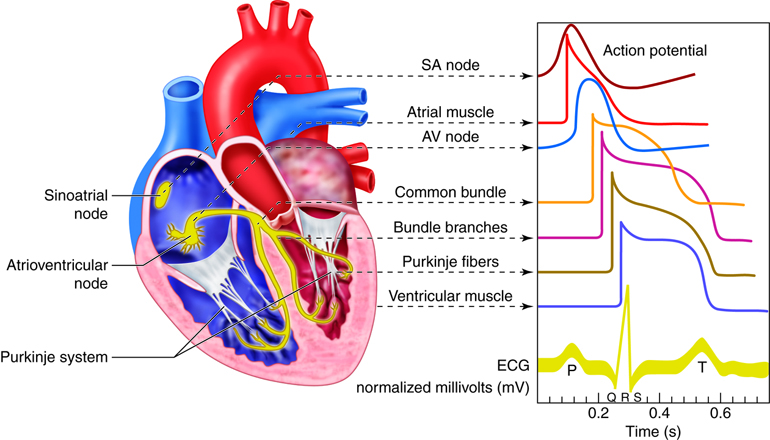
\includegraphics[width=0.9\textwidth]{figures/ecgAPs.jpg}
\caption{Action potentials recorded from different cells in the heart and their relation to the events recorded on the ECG. Image credit: Rasel Hossain Md via Wikimedia Commons, CC BY-SA 4.0.}
\label{fig:ecgAPs}
\end{figure}% 

As multiple cells in the same region of the heart depolarize, excite neighboring cells, and then repolarize, individual electrical dipoles are created which can then be summed to give us the net electrical dipole \citep{mohrman2006cardiovascular}. For example, as excitation is initiated and then spreads throughout the atria, the net electrical dipole points towards the positive ends of the leads, producing a positive deflection on the ECG. We can thus relate the different waves observed in the ECG to activity within the atria and ventricles during different phases of the cardiac cycle (Fig. \ref{fig:ecg}). 

\begin{figure}[h!]
\centering
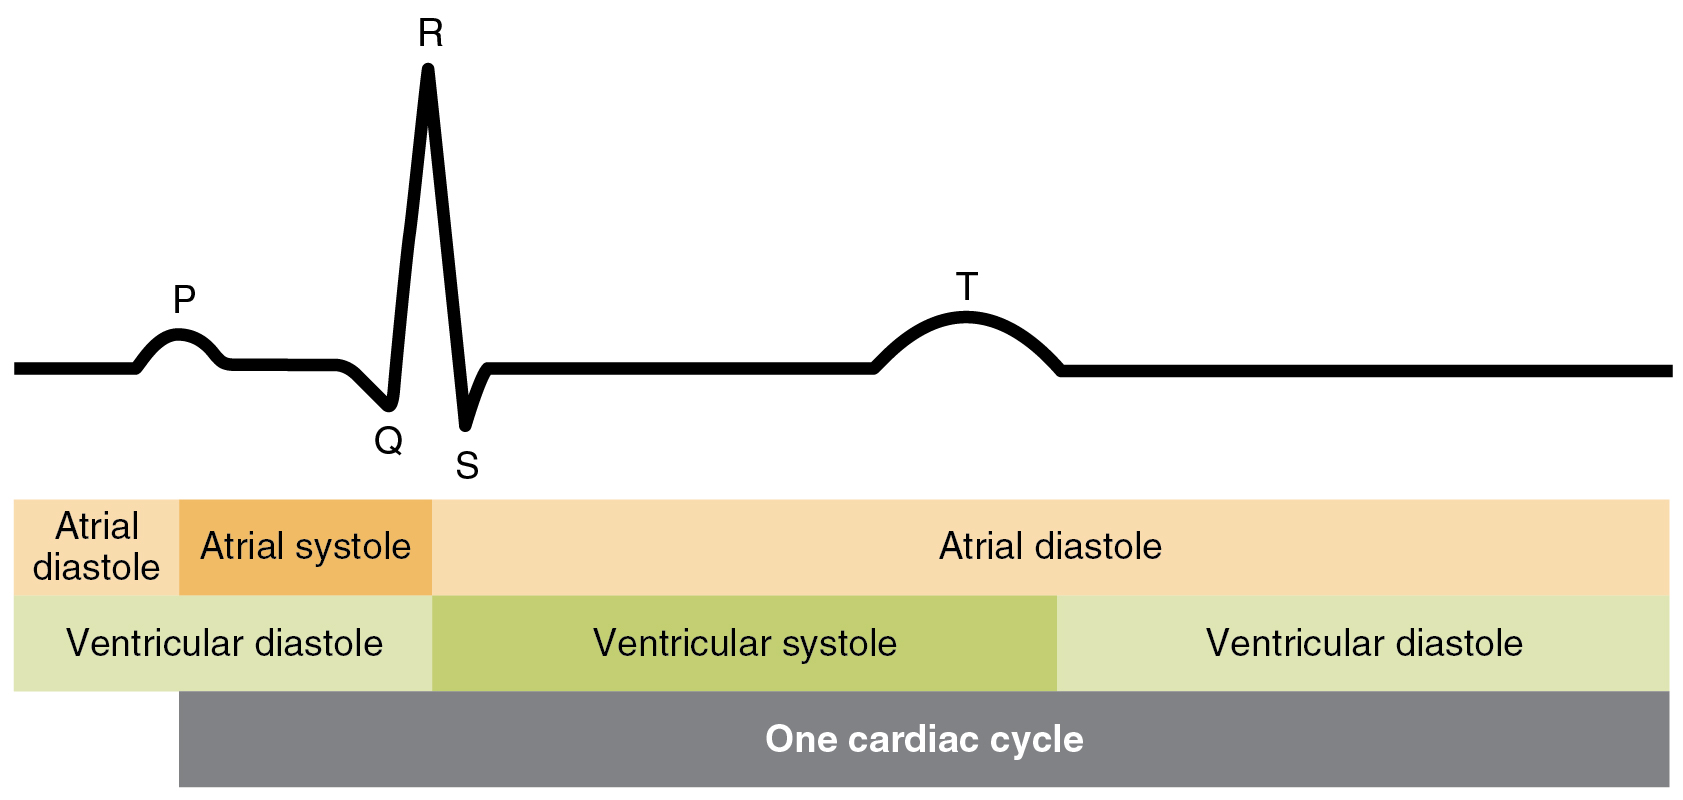
\includegraphics[width=0.9\textwidth]{figures/ECGcycle.jpg}
\caption{Image credit: Left: OpenStax College \citep{openStaxCycle}, CC BY.}
\label{fig:ecg}
\end{figure}% 

As we saw previously, the first event in the cardiac cycle is excitation of the nodal pacemaker cells. However, since there are very few of these cells, their activity is not sufficient to be detected with extracellular recording. The first observable ECG event is called the P wave, which corresponds to depolarization of the atria \citep{CVphys,mohrman2006cardiovascular,openStaxElectrical}. Atrial systole begins around the peak of the P wave (Fig. \ref{fig:ecg}) and the atria contract to pump blood into the ventricles. The second event is known as the QRS complex, which is characterized by a sequence of negative and positive deflections as depolarization spreads through the ventricles. Ventricular systole begins around the peak of the complex event (R) and blood is ejected from the heart. Finally, the T wave is generated as a wave of repolarization spreads through the ventricles and they enter diastole. At first it seems counteruntiuitive that repolarization should produce a positive deflection. However, it makes sense if we consider the order in which ventricular cells repolarize: the last to be excited are the first to relax \citep{CVphys,mohrman2006cardiovascular}. So, while the electrical dipoles are reversed, so is the direction of wave propagation. 

Measuring the intervals between electrical events observed in the ECG is useful for diagnostic purposes \citep{CVphys,mohrman2006cardiovascular,openStaxElectrical}. For example, the PR interval indicates the time it takes for electrical signals to propagate from the atria through the conduction system to the ventricles. Deviation from the normal interval range is seen in clinical conditions involving problems with electrical conduction, such as first-degree heart block. The ST segment represents the time elapsed between ventricular depolarization (i.e., plateau phase) and the beginning of repolarization. ST segment elevation is one of the primary indicators of a heart attack \citep{CVphys,mohrman2006cardiovascular,openStaxElectrical}. 

\subsection*{Study questions}

\begin{enumerate}
    \item How would you calculate the cardiac frequency from an ECG recording?
    \item What would it mean if you saw changes in the amplitude of one or more of the ECG waves?
    \item How do you think exercise will affect the ECG recording? 
\end{enumerate}

\section*{PROCEDURE}
Before beginning, make sure you have all the necessary equipment and have installed the Backyard
Brains recording software on your computer. The following steps will guide you in setting up the equipment and carrying out recordings.

\subsection*{1. Setup ECG recordings}

The Heart and Brain Spikershield comes fully assembled and ready to record. All you have to do is connect the cables and electrodes. 

\begin{enumerate}
    \item Turn on the Heart and Brain Spikershield by connecting one end of the blue cable into the device and the other end into the USB port of your computer; you should see a light flash to indicate the device is working
    \item Connect the orange cable to its corresponding port on the Heart and Brain Spikershield
    \item Place the two recording electrodes, either on the inner wrists or across the chest
    \item Place another surface electrode on the back of your hand or over your hip bone to act as a reference
        
        \begin{figure}[h!]
        \centering
        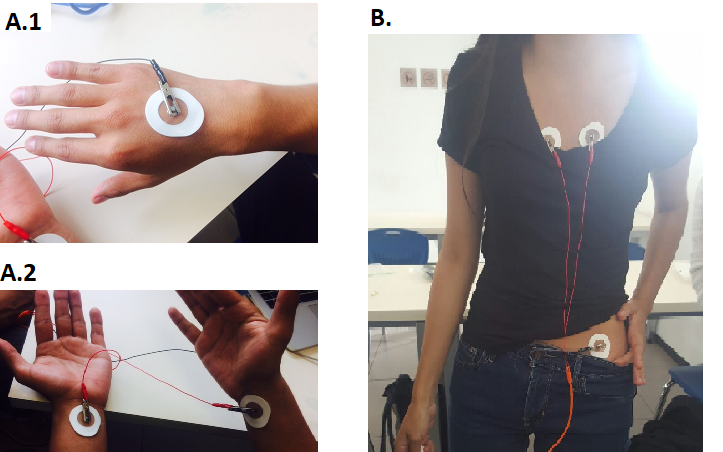
\includegraphics[width=0.6\textwidth]{figures/ecgConfig.png}
        \caption{Electrode placement for ECG. Recording electrodes can
          be placed either on the wrists or across the chest, and the
          reference electrode placed on the back of the hand or over
          the hip bone.}
        \label{fig:config}
        \end{figure}% 
    \item Connect each of the red aligator clips on the end of the orange cable to one of the surface electrodes on the wrists or chest; avoid entangling the cables
    \item Connect the black aligator clip to the reference electrode on your hand or hip
    \item To avoid noise artifacts, ensure that no clothing is touching the electrodes or brushing against the cables during recording; this is especially important if electrodes are placed on the chest
\end{enumerate}
 
\subsection*{1. Test ECG recordings}

\begin{enumerate}
    \item Open the Backyard Brains recording software and explore the controls and settings (for more info on software use, see \cite{spikeRecorder})
    \item When first connecting, you will likely see just noise; press the Config button to access the controls
    \item Ask the subject to hold still and breathe normally
    \item Verify that the principal ECG events, i.e. the P, QRS, and T waves, can be observed; at any time you can adjust the time window or signal gain to improve visualization of the recording
    \item Try saving a recording to your computer (format will be .wav)
\end{enumerate}

\begin{figure}[h!]
\centering
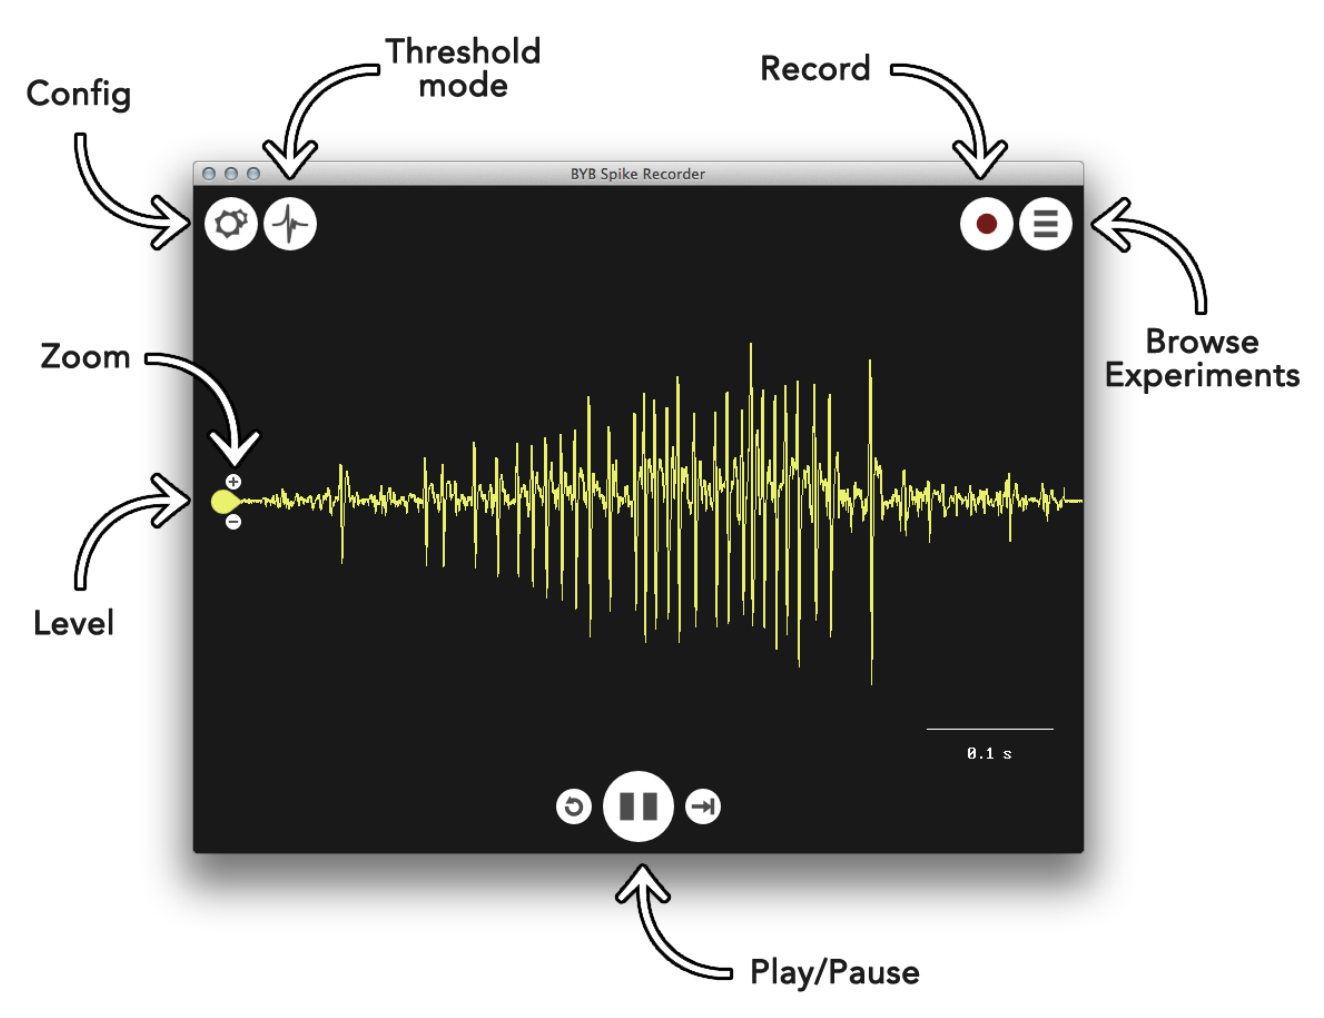
\includegraphics[width=0.8\textwidth]{figures/BBrecorder.png}
\caption{Recording software interface. Image credit: Backyard Brains, CC BY SA}
\label{fig:recorder}
\end{figure}

\subsection*{3. Collect ECG data}
\begin{enumerate}
\item Make sure the ECG is ready to record and subject is in resting position
\item When the subject is ready, press record on the Backyard Brains software interface
\item The subject should remain as still as possible during the recording to avoid generating movement artifacts
\item Record the baseline ECG for 1-2 minutes
\item Terminate the recording and save the data to your computer; use a file name that indicates the recording was taken at rest
\item ECGs should be saved and exported in .wav format for analysis
\item Disconnect the device from the computer and disconnect the alligator clips but leave the surface electrodes in place
\item Ask the subject to perform at least 5 minutes of physical activity; this could include jogging in place, pushups, or climbing stairs   
\item Once the subject has completed the physical activity, reconnect the alligator clips to the electrodes
\item Reconnect the device to the computer; you will likely have to reconfigure the device in settings to reestablish the ECG signal
\item Press record on the Backyard Brains software interface
\item Record the ECG post-exercise for 1-2 minutes
\item Terminate the recording and save the data to your computer; use a file name that indicates the recording was taken after exercise
\item Repeat the above steps in at least 3-5 subjects to compare results
\item Exercise duration and intensity can also be varied to explore the effects
\end{enumerate}

\section*{ACKNOWLEDGMENTS}
This work was supported by UNAM-DGAPA-PAPIME PE213817 and PE213219.

% BIBLIOGRAPHY
\renewcommand\refname{REFERENCES}
\renewcommand{\markboth}[2]{}%
\begin{footnotesize}
\bibliography{ECG}
\end{footnotesize}

\end{document}
